\subparagraph{Задание 4.14}

\textbf{Условие}:
Изменить содержимое регистра CX на величину, меньшую на 2 единицы (\path{Data->Evaluate/Modify->Expression=cx}, New Value=cx-2). Выполнить пошагово (F7) программу до конца. Что изменилось? Объяснить в отчете.

\textbf{Решение}:

\begin{figure}[!htp]
    \centering
    \begin{minipage}{0.32\textwidth}
        \centering
        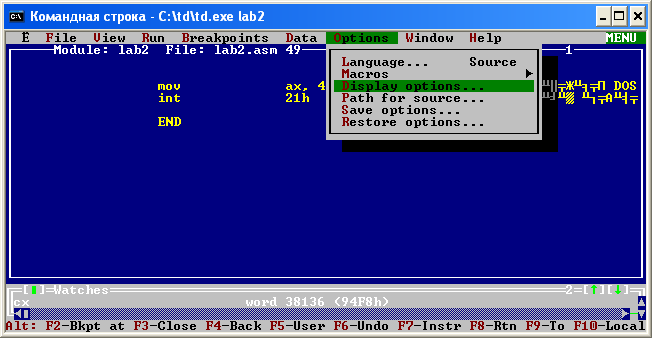
\includegraphics[width=.99\linewidth]
            {../_INCLUDES/task-4-14/1.png}
        \caption{1) }
        \label{fig:task_4_14__1}
    \end{minipage}
    \begin {minipage}{0.32\textwidth}
        \centering
        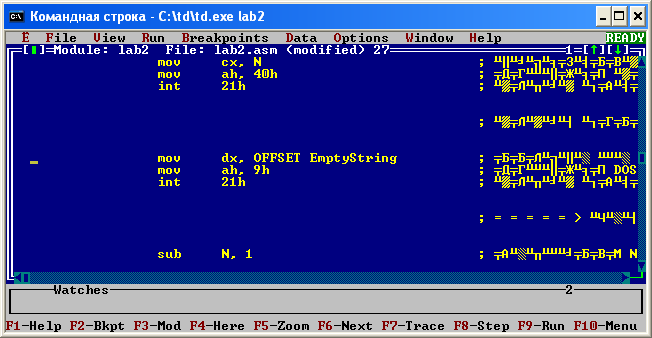
\includegraphics[width=.99\linewidth]
            {../_INCLUDES/task-4-14/2.png}
        \caption{2) }
        \label{fig:task_4_14__2}
    \end{minipage}
    \begin {minipage}{0.32\textwidth}
        \centering
        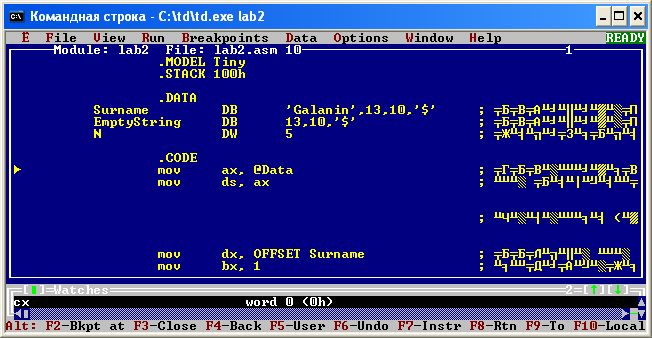
\includegraphics[width=.99\linewidth]
            {../_INCLUDES/task-4-14/3.png}
        \caption{3) }
        \label{fig:task_4_14__3}
    \end{minipage}
\end{figure}

На рисунке~\ref{fig:task_4_14__1} (стр.~\pageref{fig:task_4_14__1})
запушен Turbo Debugger после команды
\textbf{C:\textbackslash\/td\textbackslash\/td.exe lab2}.

Нужно добавить в Watches регистр cx.
Переходим в меню клавишей \textbf{F10}.
Выбираю пункт \textbf{View}.
Жму \textbf{Enter}.
Выбираю пункт \textbf{Watches}.
Жму \textbf{Enter}.
Рисунок~\ref{fig:task_4_14__2} (стр.~\pageref{fig:task_4_14__2}).

Жму \textbf{c}.
Открывается окно.
Дописываю \textbf{x} в поле \textbf{Enter expression to watch}.
Рисунок~\ref{fig:task_4_14__3} (стр.~\pageref{fig:task_4_14__3}).

\begin{figure}[!htp]
    \centering
    \begin{minipage}{0.32\textwidth}
        \centering
        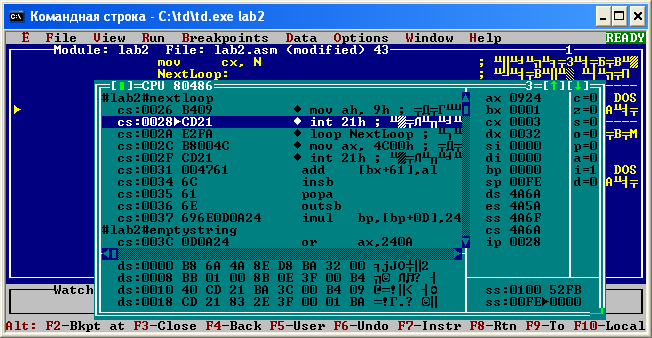
\includegraphics[width=.99\linewidth]
            {../_INCLUDES/task-4-14/4.png}
        \caption{4) }
        \label{fig:task_4_14__4}
    \end{minipage}
    \begin {minipage}{0.32\textwidth}
        \centering
        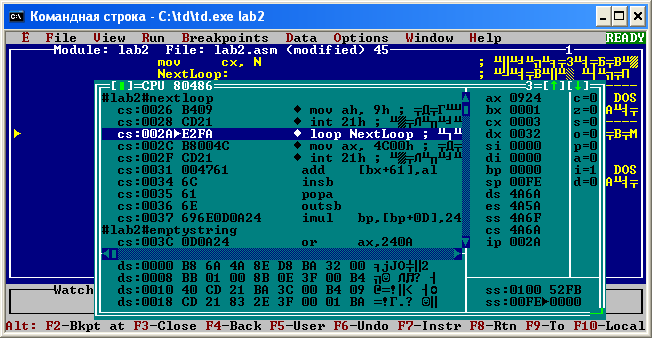
\includegraphics[width=.99\linewidth]
            {../_INCLUDES/task-4-14/5.png}
        \caption{5) }
        \label{fig:task_4_14__5}
    \end{minipage}
    \begin {minipage}{0.32\textwidth}
        \centering
        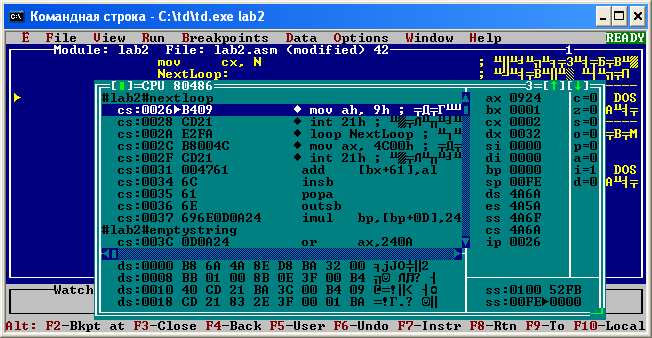
\includegraphics[width=.99\linewidth]
            {../_INCLUDES/task-4-14/6.png}
        \caption{6) }
        \label{fig:task_4_14__6}
    \end{minipage}
\end{figure}

В поле Wathes текст \textbf{сх word 0 (0h)}.
Это значит, что регистр cx имеет значение 0.
В Turbo Debugger стрелка на строке \textbf{mov ax, @Data}.
Жмём \textbf{F7}.
Рисунок~\ref{fig:task_4_14__4} (стр.~\pageref{fig:task_4_14__4}).

В поле Wathes текст \textbf{сх word 0 (0h)}.
Это значит, что регистр cx имеет значение 0.
В Turbo Debugger стрелка на строке \textbf{mov ds, ax}.
Жмём \textbf{F7}.
Рисунок~\ref{fig:task_4_14__5} (стр.~\pageref{fig:task_4_14__5}).


В поле Wathes текст \textbf{сх word 0 (0h)}.
Это значит, что регистр cx имеет значение 0.
В Turbo Debugger стрелка на строке \textbf{mov dx, OFFSET Surname}.
Жмём \textbf{F7}.
Рисунок~\ref{fig:task_4_14__6} (стр.~\pageref{fig:task_4_14__6}).

\begin{figure}[!htp]
    \centering
    \begin{minipage}{0.32\textwidth}
        \centering
        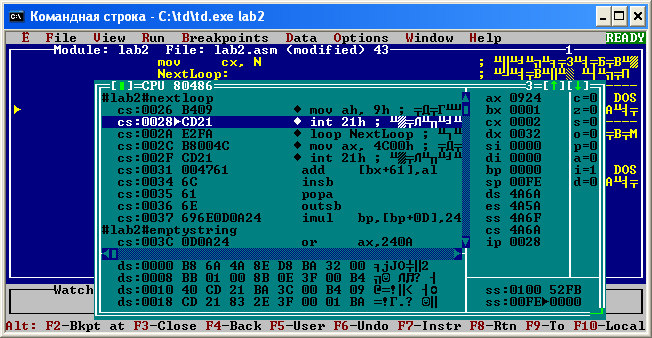
\includegraphics[width=.99\linewidth]
            {../_INCLUDES/task-4-14/7.png}
        \caption{7) }
        \label{fig:task_4_14__7}
    \end{minipage}
    \begin {minipage}{0.32\textwidth}
        \centering
        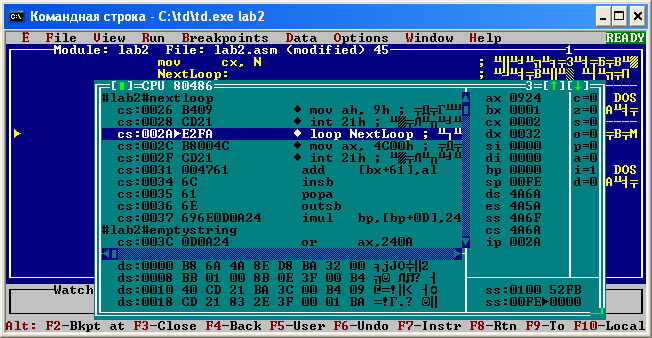
\includegraphics[width=.99\linewidth]
            {../_INCLUDES/task-4-14/8.png}
        \caption{8) }
        \label{fig:task_4_14__8}
    \end{minipage}
    \begin {minipage}{0.32\textwidth}
        \centering
        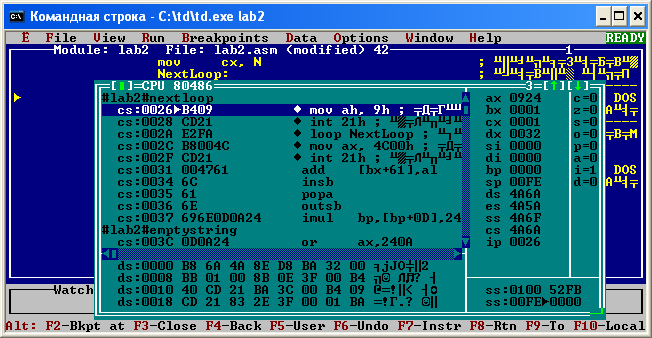
\includegraphics[width=.99\linewidth]
            {../_INCLUDES/task-4-14/9.png}
        \caption{9) }
        \label{fig:task_4_14__9}
    \end{minipage}
\end{figure}

В поле Wathes текст \textbf{word 0 (0h)}.
Это значит, что регистр cx имеет значение 0.
В Turbo Debugger стрелка на строке \textbf{mov bx, 1}.
Жмём \textbf{F7}.
Рисунок~\ref{fig:task_4_14__7} (стр.~\pageref{fig:task_4_14__7}).


В поле Wathes текст \textbf{word 0 (0h)}.
Это значит, что регистр cx имеет значение 0.
В Turbo Debugger стрелка на строке \textbf{mov cx, N}.
Жмём \textbf{F7}. 
Рисунок~\ref{fig:task_4_14__8} (стр.~\pageref{fig:task_4_14__8}).

В поле Wathes текст \textbf{word 5 (5h)}.
Это значит, что регистр cx имеет значение 5.
В Turbo Debugger стрелка на строке \textbf{mov ah, 40h}.
Жмём \textbf{F7}. 
Рисунок~\ref{fig:task_4_14__9} (стр.~\pageref{fig:task_4_14__9}).

\begin{figure}[!htp]
    \centering
    \begin{minipage}{0.32\textwidth}
        \centering
        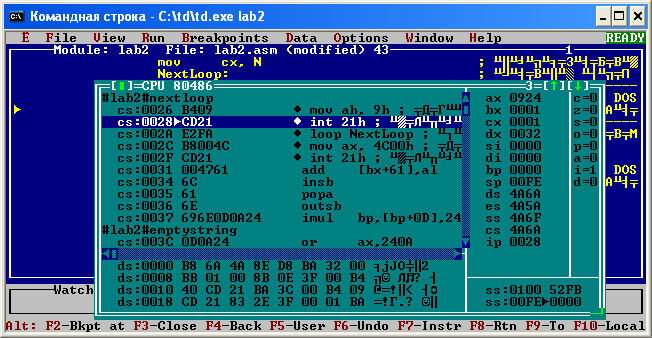
\includegraphics[width=.99\linewidth]
            {../_INCLUDES/task-4-14/10.png}
        \caption{10) }
        \label{fig:task_4_14__10}
    \end{minipage}
    \begin {minipage}{0.32\textwidth}
        \centering
        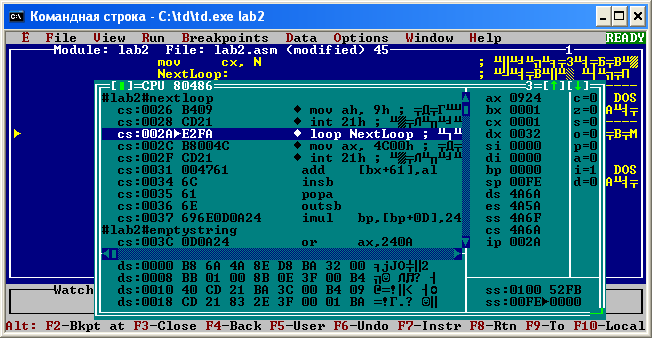
\includegraphics[width=.99\linewidth]
            {../_INCLUDES/task-4-14/11.png}
        \caption{11) }
        \label{fig:task_4_14__11}
    \end{minipage}
    \begin {minipage}{0.32\textwidth}
        \centering
        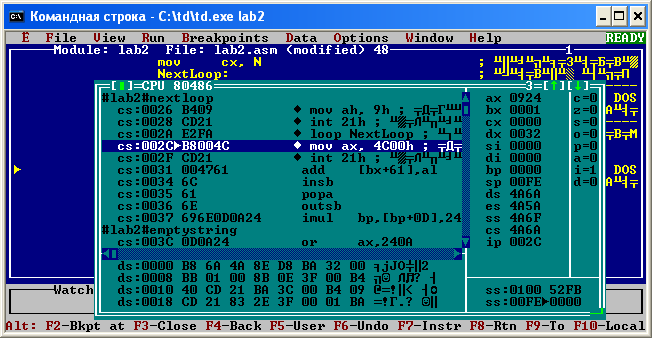
\includegraphics[width=.99\linewidth]
            {../_INCLUDES/task-4-14/12.png}
        \caption{12) }
        \label{fig:task_4_14__12}
    \end{minipage}
\end{figure}

В поле Wathes текст \textbf{word 5 (5h)}.
Это значит, что регистр cx имеет значение 5.
В Turbo Debugger стрелка на строке \textbf{int 21h}.
Жмём \textbf{F7}.
Рисунок~\ref{fig:task_4_14__10} (стр.~\pageref{fig:task_4_14__10}).

В поле Wathes текст \textbf{word 5 (5h)}.
Это значит, что регистр cx имеет значение 5.
В Turbo Debugger стрелка на строке \textbf{mov dx, OFFSET EmptyString}.
Жмём \textbf{F7}.
Рисунок~\ref{fig:task_4_14__11} (стр.~\pageref{fig:task_4_14__11}).

В поле Wathes текст \textbf{word 5 (5h)}.
Это значит, что регистр cx имеет значение 5.
В Turbo Debugger на строке \textbf{mov ah, 9h}.
Жмём \textbf{F7}.
Рисунок~\ref{fig:task_4_14__12} (стр.~\pageref{fig:task_4_14__12}).

\begin{figure}[!htp]
    \centering
    \begin{minipage}{0.32\textwidth}
        \centering
        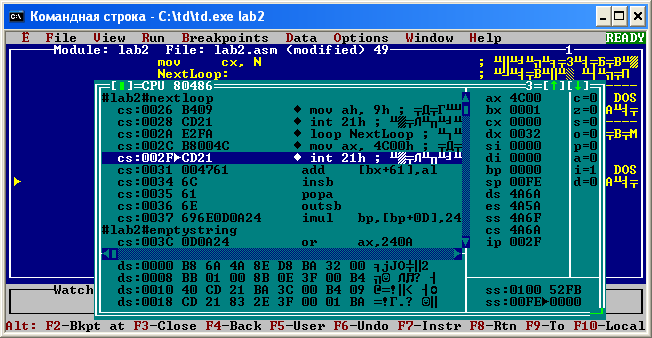
\includegraphics[width=.99\linewidth]
            {../_INCLUDES/task-4-14/13.png}
        \caption{13) }
        \label{fig:task_4_14__13}
    \end{minipage}
    \begin {minipage}{0.32\textwidth}
        \centering
        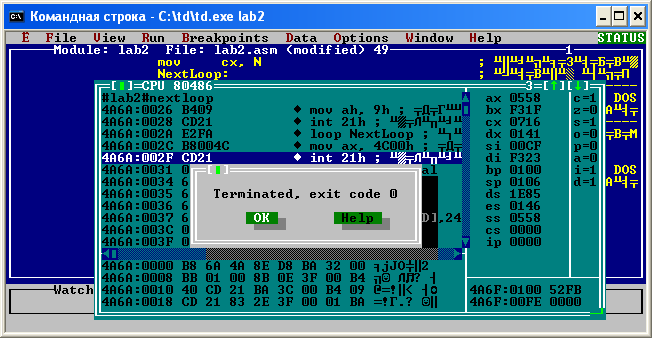
\includegraphics[width=.99\linewidth]
            {../_INCLUDES/task-4-14/14.png}
        \caption{14) }
        \label{fig:task_4_14__14}
    \end{minipage}
    \begin {minipage}{0.32\textwidth}
        \centering
        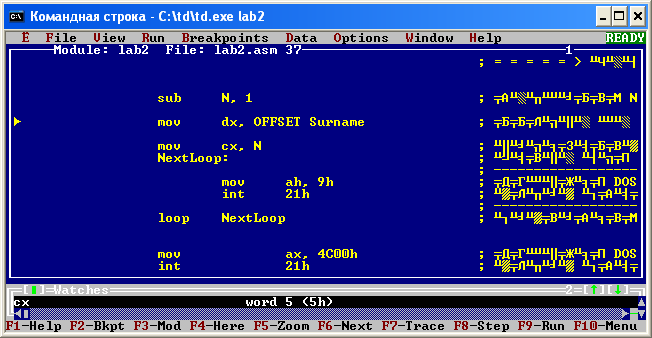
\includegraphics[width=.99\linewidth]
            {../_INCLUDES/task-4-14/15.png}
        \caption{15) }
        \label{fig:task_4_14__15}
    \end{minipage}
\end{figure}

В поле Wathes текст \textbf{word 5 (5h)}.
Это значит, что регистр cx имеет значение 5.
В Turbo Debugger стрелка на строке \textbf{int 21h}.
Жмём \textbf{F7}.
Рисунок~\ref{fig:task_4_14__13} (стр.~\pageref{fig:task_4_14__13}).

В поле Wathes текст \textbf{word 5 (5h)}.
Это значит, что регистр cx имеет значение 5.
В Turbo Debugger на строке \textbf{sub N, 1}.
\textbf{sub} от первого элемента отнимает второй элемент.
N было 5, (5-1 = 4) а стало 4, но в сх пока 5.
Жмём \textbf{F7}.
Рисунок~\ref{fig:task_4_14__14} (стр.~\pageref{fig:task_4_14__14}).

В поле Wathes текст \textbf{word 5 (5h)}.
Это значит, что регистр cx имеет значение 5.
В Turbo Debugger стрелка на строке \textbf{mov dx, OFFSET Surname}.
Жмём \textbf{F7}.
Рисунок~\ref{fig:task_4_14__15} (стр.~\pageref{fig:task_4_14__15}).

\begin{figure}[!htp]
    \centering
    \begin{minipage}{0.32\textwidth}
        \centering
        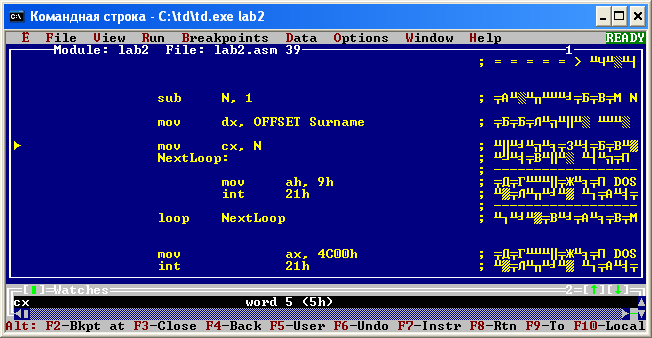
\includegraphics[width=.99\linewidth]
            {../_INCLUDES/task-4-14/16.png}
        \caption{16) }
        \label{fig:task_4_14__16}
    \end{minipage}
    \begin {minipage}{0.32\textwidth}
        \centering
        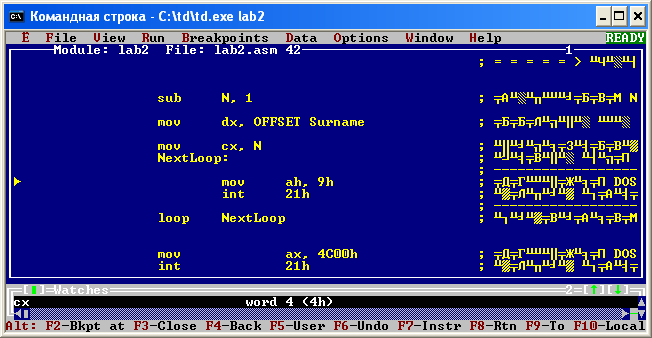
\includegraphics[width=.99\linewidth]
            {../_INCLUDES/task-4-14/17.png}
        \caption{17) }
        \label{fig:task_4_14__17}
    \end{minipage}
    \begin {minipage}{0.32\textwidth}
        \centering
        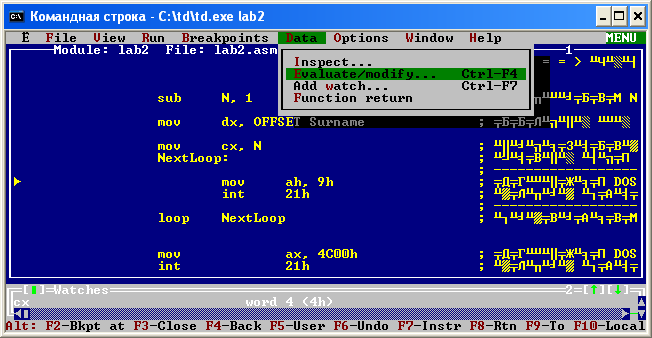
\includegraphics[width=.99\linewidth]
            {../_INCLUDES/task-4-14/18.png}
        \caption{18) }
        \label{fig:task_4_14__18}
    \end{minipage}
\end{figure}

В поле Wathes текст \textbf{word 5 (5h)}.
Это значит, что регистр cx имеет значение 5.
В Turbo Debugger стрелка на строке \textbf{mov cx, N}.
В сх запишется N, а так как N равен 4, то сх будет 4.
Жмём \textbf{F7}.
Рисунок~\ref{fig:task_4_14__16} (стр.~\pageref{fig:task_4_14__16}).

В поле Wathes текст \textbf{word 4 (4h)}.
Это значит, что регистр cx имеет значение 4.
В Turbo Debugger стрелка на строке \textbf{mov ah, 9h}.
Рисунок~\ref{fig:task_4_14__17} (стр.~\pageref{fig:task_4_14__17}).
Мы находимся в цикле.
Значение сх уже было присвоено.
Можем приступать изменять значение регистра сх.
Цикл может содержать тысячи операций (сх = 1000).
Например, мы хотим поменять эти итерации (cx) на другое число.
Это мы будем делать дальше.

Жмем \textbf{F10} - и попадаем в меню.
В меню выбираем пукнт \textbf{Data}.
В пункте \textbf{Data} выбираю пункт \textbf{Evaluate/modify...}.
Рисунок~\ref{fig:task_4_14__18} (стр.~\pageref{fig:task_4_14__18}).

\begin{figure}[!htp]
    \centering
    \begin{minipage}{0.32\textwidth}
        \centering
        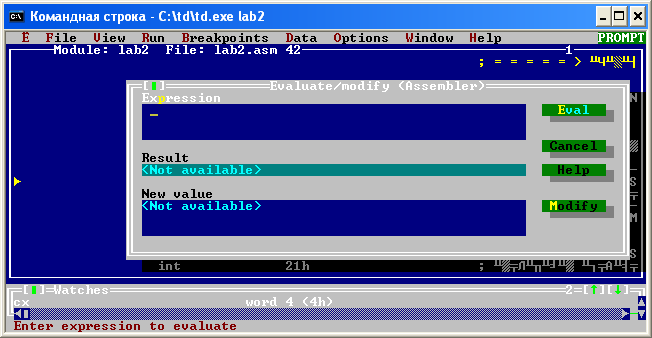
\includegraphics[width=.99\linewidth]
            {../_INCLUDES/task-4-14/19.png}
        \caption{19) }
        \label{fig:task_4_14__19}
    \end{minipage}
    \begin {minipage}{0.32\textwidth}
        \centering
        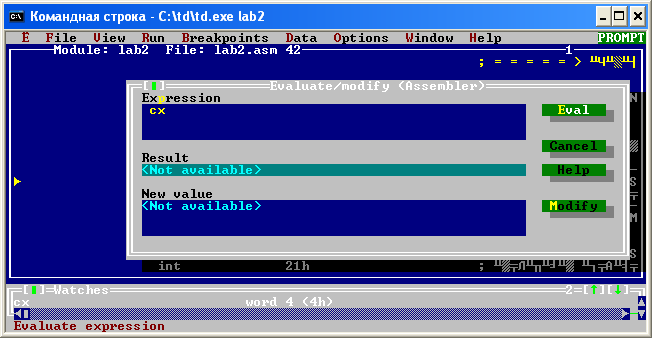
\includegraphics[width=.99\linewidth]
            {../_INCLUDES/task-4-14/20.png}
        \caption{20) }
        \label{fig:task_4_14__20}
    \end{minipage}
    \begin {minipage}{0.32\textwidth}
        \centering
        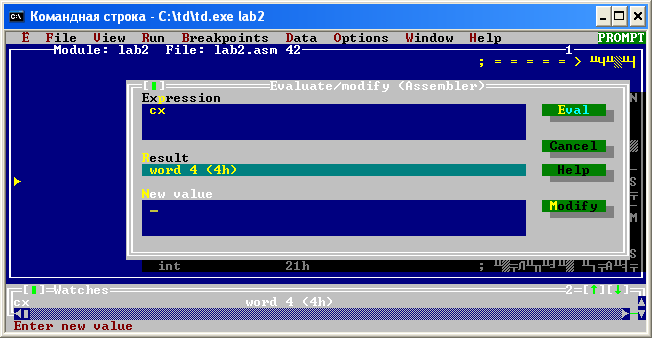
\includegraphics[width=.99\linewidth]
            {../_INCLUDES/task-4-14/21.png}
        \caption{21) }
        \label{fig:task_4_14__21}
    \end{minipage}
\end{figure}

Открылось окошко, к котором можем узнать значение регистра, и тут же изменить его.
Рисунок~\ref{fig:task_4_14__19} (стр.~\pageref{fig:task_4_14__19}).

В поле \textbf{Expression} ввожу регистр \textbf{cx}.
Табом выбираю кнопку \textbf{Eval}.
Жму \textbf{Enter}.
Рисунок~\ref{fig:task_4_14__20} (стр.~\pageref{fig:task_4_14__20}).

В поле \textbf{Result} появился текст \textbf{word 4 (4h)}.
Это значит, что в регистр cx имеет значение 4.
Рисунок~\ref{fig:task_4_14__21} (стр.~\pageref{fig:task_4_14__21}).

\begin{figure}[!htp]
    \centering
    \begin{minipage}{0.32\textwidth}
        \centering
        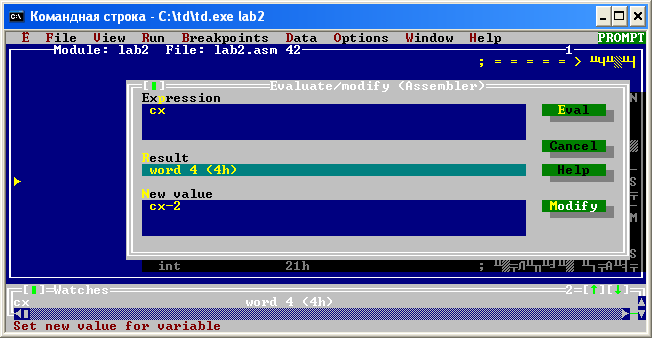
\includegraphics[width=.99\linewidth]
            {../_INCLUDES/task-4-14/22.png}
        \caption{22) }
        \label{fig:task_4_14__22}
    \end{minipage}
    \begin {minipage}{0.32\textwidth}
        \centering
        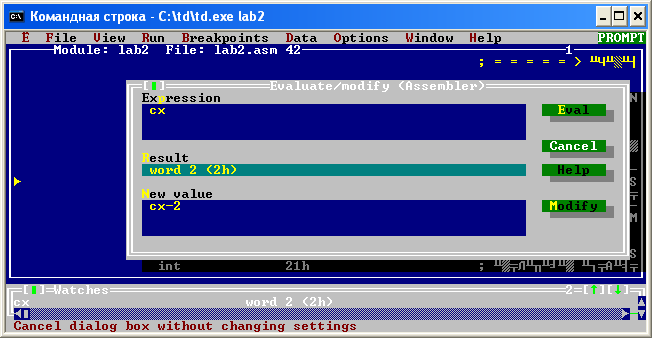
\includegraphics[width=.99\linewidth]
            {../_INCLUDES/task-4-14/23.png}
        \caption{23) }
        \label{fig:task_4_14__23}
    \end{minipage}
    \begin {minipage}{0.32\textwidth}
        \centering
        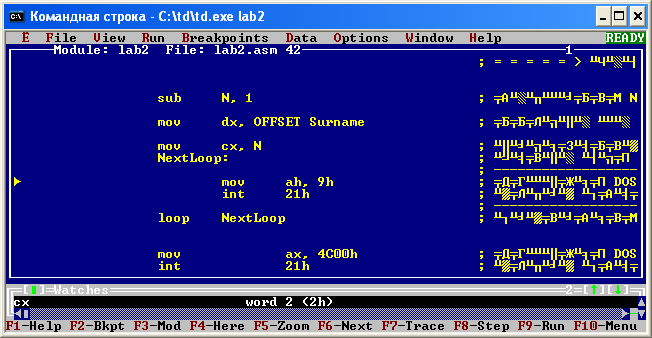
\includegraphics[width=.99\linewidth]
            {../_INCLUDES/task-4-14/24.png}
        \caption{24) }
        \label{fig:task_4_14__24}
    \end{minipage}
\end{figure}

В поле \textbf{New value} ввожу cx-2.
Выбираю табом кнопку \textbf{Modify}.
Значение поля \textbf{Result} пока \textbf{word 4 4 (4h)}.
То есть регист cx пока имеет значение 4.
Жму \textbf{Enter}.
Рисунок~\ref{fig:task_4_14__22} (стр.~\pageref{fig:task_4_14__22}).

Значение поля \textbf{Result} имеет значение \textbf{word 2 (2h)}.
Это значит, что регистр сх имеет значение 2.
Выбираю табом кнопку \textbf{Cancel}.
Жму \textbf{Enter}.
Рисунок~\ref{fig:task_4_14__23} (стр.~\pageref{fig:task_4_14__23}).

Вернулись обратно к коду в Turbo Debugger.
Поле Watches имеет значение \textbf{word 2 (2h)}.
Это значит, что регистр cx имеет значение 2.
В Turbo Debugger стрелка на строке \textbf{mov ah, 9h}.
Жмем \textbf{F7}.
Рисунок~\ref{fig:task_4_14__24} (стр.~\pageref{fig:task_4_14__24}).

\begin{figure}[!htp]
    \centering
    \begin{minipage}{0.32\textwidth}
        \centering
        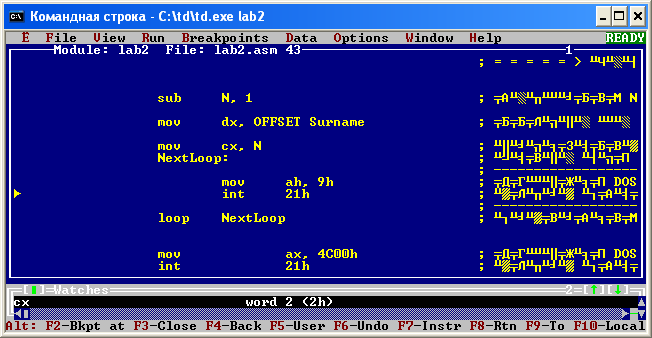
\includegraphics[width=.99\linewidth]
            {../_INCLUDES/task-4-14/25.png}
        \caption{25) }
        \label{fig:task_4_14__25}
    \end{minipage}
    \begin {minipage}{0.32\textwidth}
        \centering
        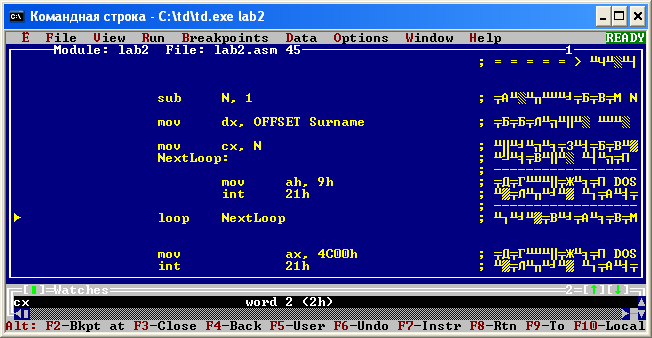
\includegraphics[width=.99\linewidth]
            {../_INCLUDES/task-4-14/26.png}
        \caption{26) }
        \label{fig:task_4_14__26}
    \end{minipage}
    \begin {minipage}{0.32\textwidth}
        \centering
        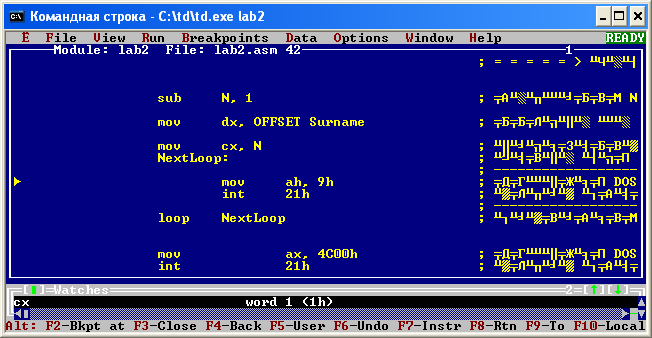
\includegraphics[width=.99\linewidth]
            {../_INCLUDES/task-4-14/27.png}
        \caption{27) }
        \label{fig:task_4_14__27}
    \end{minipage}
\end{figure}

Поле Watches имеет значение \textbf{word 2 (2h)}.
Это значит, что регистр cx имеет значение 2.
В Turbo Debugger стрелка на строке \textbf{int 21h}.
Жмем \textbf{F7}.
Рисунок~\ref{fig:task_4_14__25} (стр.~\pageref{fig:task_4_14__25}).

Поле Watches имеет значение \textbf{word 2 (2h)}.
Это значит, что регистр cx имеет значение 2.
В Turbo Debugger стрелка на строке \textbf{loop NextLoop}.
Жмем \textbf{F7}.
Рисунок~\ref{fig:task_4_14__26} (стр.~\pageref{fig:task_4_14__26}).

В Turbo Debugger стрелка на строке \textbf{mov ah, 9h}.
Видем, что цикл идёт по новой.
Поле Watches имеет значение \textbf{word 1 (1h)}.
Это значит, что регистр cx имеет значение 1.
Жмем \textbf{F7}.
Рисунок~\ref{fig:task_4_14__27} (стр.~\pageref{fig:task_4_14__27}).

\begin{figure}[!htp]
    \centering
    \begin{minipage}{0.32\textwidth}
        \centering
        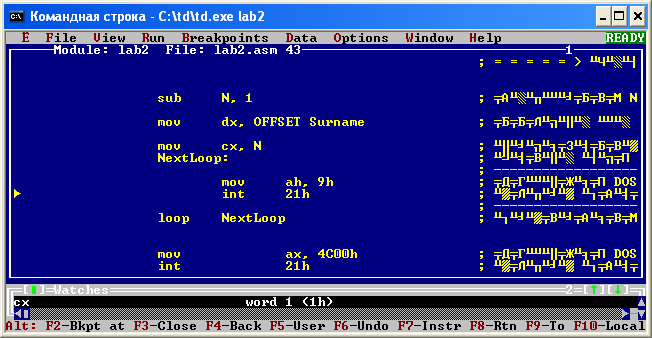
\includegraphics[width=.99\linewidth]
            {../_INCLUDES/task-4-14/28.png}
        \caption{28) }
        \label{fig:task_4_14__28}
    \end{minipage}
    \begin {minipage}{0.32\textwidth}
        \centering
        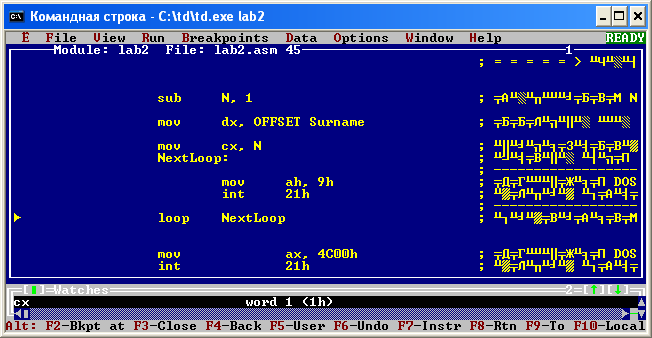
\includegraphics[width=.99\linewidth]
            {../_INCLUDES/task-4-14/29.png}
        \caption{29) }
        \label{fig:task_4_14__29}
    \end{minipage}
    \begin {minipage}{0.32\textwidth}
        \centering
        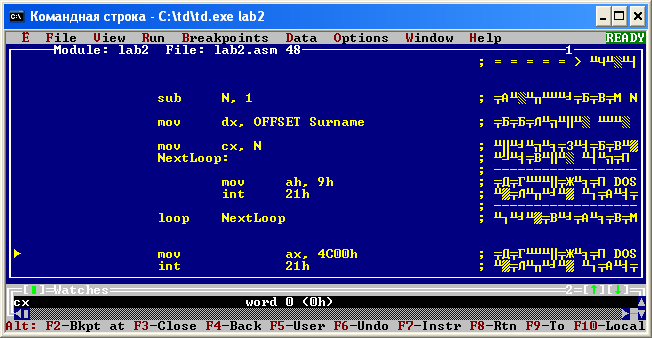
\includegraphics[width=.99\linewidth]
            {../_INCLUDES/task-4-14/30.png}
        \caption{30) }
        \label{fig:task_4_14__30}
    \end{minipage}
\end{figure}

Поле Watches имеет значение \textbf{word 1 (1h)}.
Это значит, что регистр cx имеет значение 1.
В Turbo Debugger стрелка на строке \textbf{int 21h}.
Жмем \textbf{F7}.
Рисунок~\ref{fig:task_4_14__28} (стр.~\pageref{fig:task_4_14__28}).

Поле Watches имеет значение \textbf{word 1 (1h)}.
Это значит, что регистр cx имеет значение 1.
В Turbo Debugger стрелка на строке \textbf{loop NextLoop}.
Жмем \textbf{F7}.
Рисунок~\ref{fig:task_4_14__29} (стр.~\pageref{fig:task_4_14__29}).

Поле Watches имеет значение \textbf{word 0 (0h)}.
Это значит, что регистр cx имеет значение 0.
То есть цикл окончен.
В Turbo Debugger стрелка на строке \textbf{mov ax, 4C00h}. Жмем \textbf{F7}.
Рисунок~\ref{fig:task_4_14__30} (стр.~\pageref{fig:task_4_14__30}).

\begin{figure}[!htp]
    \centering
    \begin{minipage}{0.32\textwidth}
        \centering
        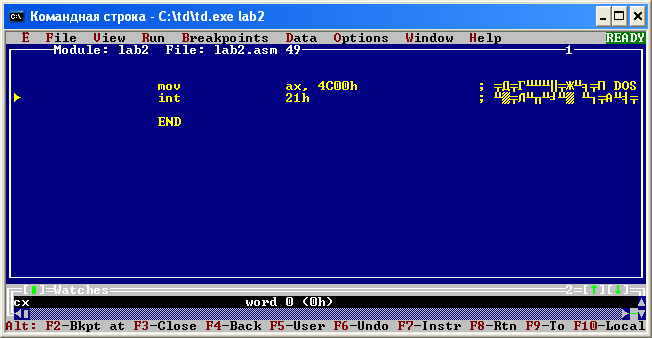
\includegraphics[width=.99\linewidth]
            {../_INCLUDES/task-4-14/31.png}
        \caption{31) }
        \label{fig:task_4_14__31}
    \end{minipage}
    \begin {minipage}{0.32\textwidth}
        \centering
        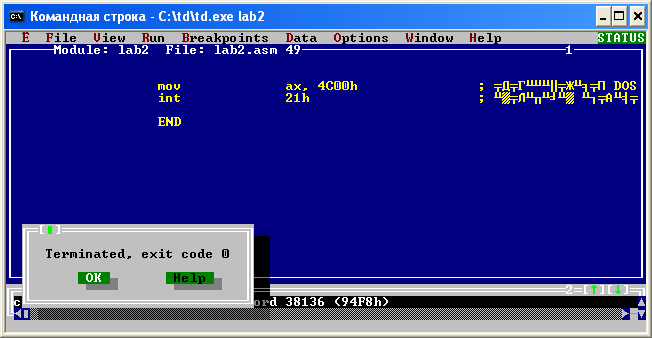
\includegraphics[width=.99\linewidth]
            {../_INCLUDES/task-4-14/32.png}
        \caption{32) }
        \label{fig:task_4_14__32}
    \end{minipage}
    \begin {minipage}{0.32\textwidth}
        \centering
        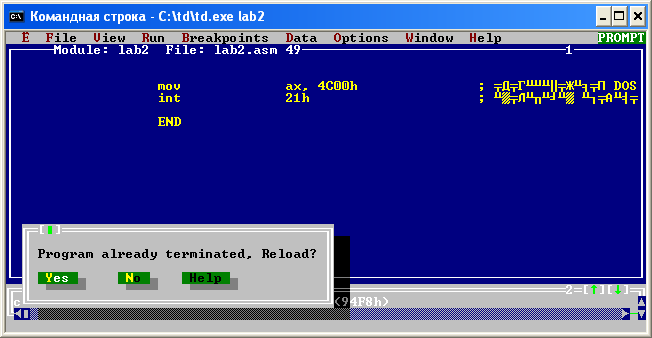
\includegraphics[width=.99\linewidth]
            {../_INCLUDES/task-4-14/33.png}
        \caption{33) }
        \label{fig:task_4_14__33}
    \end{minipage}
\end{figure}

Поле Watches имеет значение \textbf{word 0 (0h)}.
Это значит, что регистр cx имеет значение 0.
В Turbo Debugger стрелка на строке \textbf{int 21h}.
Жмем \textbf{F7}.
Рисунок~\ref{fig:task_4_14__31} (стр.~\pageref{fig:task_4_14__31}).

Turbo Debugger говорит, что программа завершена успешно с кодом 0:
\textbf{Terminated, exit code 0}.
Жмем \textbf{Enter}.
Жмем \textbf{F7}.
Рисунок~\ref{fig:task_4_14__32} (стр.~\pageref{fig:task_4_14__32}).

Turbo Debugger говорит, что программа закончена и можно начать дебаг по новой:
\textbf{Program already terminated, Reload?}
Жмем \textbf{Enter}.
Жмем \textbf{F7}.
Рисунок~\ref{fig:task_4_14__33} (стр.~\pageref{fig:task_4_14__33}).

\newpage
